\section{Theory and Analytical Model}
\label{sec:theory-and-model}

The modeled structure is an air--dielectric--air stack under normal incidence. The
dielectric is lossless and nonmagnetic, so
\begin{equation}
\mu_r=1,
\qquad
\varepsilon=\varepsilon_r\varepsilon_0.
\end{equation}

\subsection{Wave Impedance and Phase Constant}

The intrinsic impedance and phase constant inside the dielectric are
\begin{equation}
\eta_d=\sqrt{\frac{\mu_0}{\varepsilon_0\varepsilon_r}}
=\frac{\eta_0}{\sqrt{\varepsilon_r}},
\label{eq:eta-d}
\end{equation}
and
\begin{equation}
\beta_d=k_0\sqrt{\varepsilon_r}
=\frac{2\pi}{\lambda_0}\sqrt{\varepsilon_r}.
\label{eq:beta-d}
\end{equation}
At 1~GHz,
\begin{equation}
\lambda_0=\frac{c}{f_0}=299.792~\text{mm}.
\label{eq:lambda0}
\end{equation}

\subsection{Equivalent Transmission-Line Section}

The slab is represented as a lossless transmission-line section of characteristic
impedance $\eta_d$, length $d$, and load impedance $Z_L=\eta_0$. The input impedance
looking into the slab is
\begin{equation}
Z_{\mathrm{in}}=\eta_d
\frac{Z_L+j\eta_d\tan(\beta_d d)}
{\eta_d+jZ_L\tan(\beta_d d)}.
\label{eq:zin}
\end{equation}
The analytical input reflection coefficient is
\begin{equation}
\Gamma_{\mathrm{ana}}=
\frac{Z_{\mathrm{in}}-\eta_0}{Z_{\mathrm{in}}+\eta_0}.
\label{eq:gamma}
\end{equation}

\subsection{Half-Wavelength Matching Condition}

When the line length is an integer multiple of one-half wavelength in the dielectric,
the input impedance repeats the load impedance:
\begin{equation}
d=m\frac{\lambda_d}{2},
\qquad
\lambda_d=\frac{\lambda_0}{\sqrt{\varepsilon_r}}.
\label{eq:half-wave-condition}
\end{equation}
For $d=\lambda_0$,
\begin{align}
\lambda_0 &= m\frac{\lambda_0}{2\sqrt{\varepsilon_r}},\\
\sqrt{\varepsilon_r}&=\frac{m}{2},\\
\varepsilon_r&=\left(\frac{m}{2}\right)^2.
\label{eq:matching-eps}
\end{align}

\begin{table}[H]
\centering
\caption{Analytically predicted matched permittivity values for $d=\lambda_0$.}
\label{tab:predicted-minima}
\begin{tabular}{@{}ccc@{}}
\toprule
\textbf{Half-wave index $m$} & \textbf{$\sqrt{\varepsilon_r}=m/2$} & \textbf{Predicted $\varepsilon_r$} \\
\midrule
2 & 1.0 & 1.00 \\
3 & 1.5 & 2.25 \\
4 & 2.0 & 4.00 \\
5 & 2.5 & 6.25 \\
6 & 3.0 & 9.00 \\
\bottomrule
\end{tabular}
\end{table}

Figure~\ref{fig:analytical-gamma} shows the regenerated ideal analytical response.
The zeros occur at the values in Table~\ref{tab:predicted-minima}. The analytical
phase is mathematically ill-conditioned at an exact zero because a complex number at
the origin has no unique phase.

\begin{figure}[H]
    \centering
    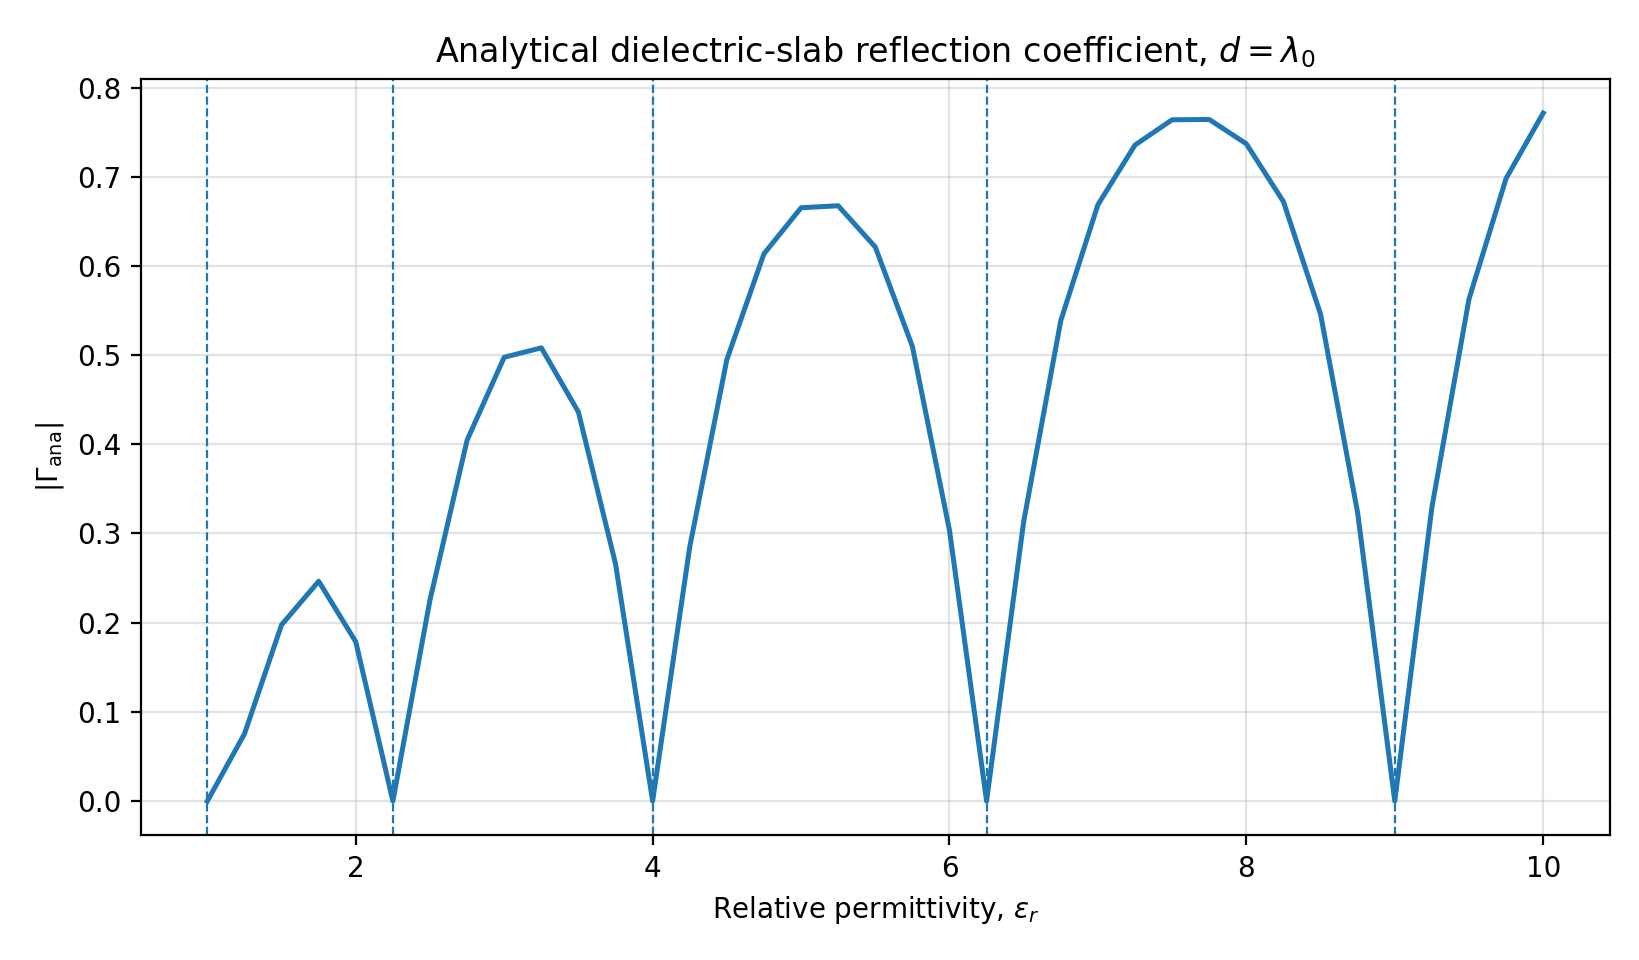
\includegraphics[width=0.88\textwidth]{figures/analytical/analytical_gamma_vs_eps.png}
    \caption{Regenerated analytical reflection magnitude for the ideal
    air--dielectric--air slab with $d=\lambda_0$.}
    \label{fig:analytical-gamma}
\end{figure}

\begin{figure}[H]
    \centering
    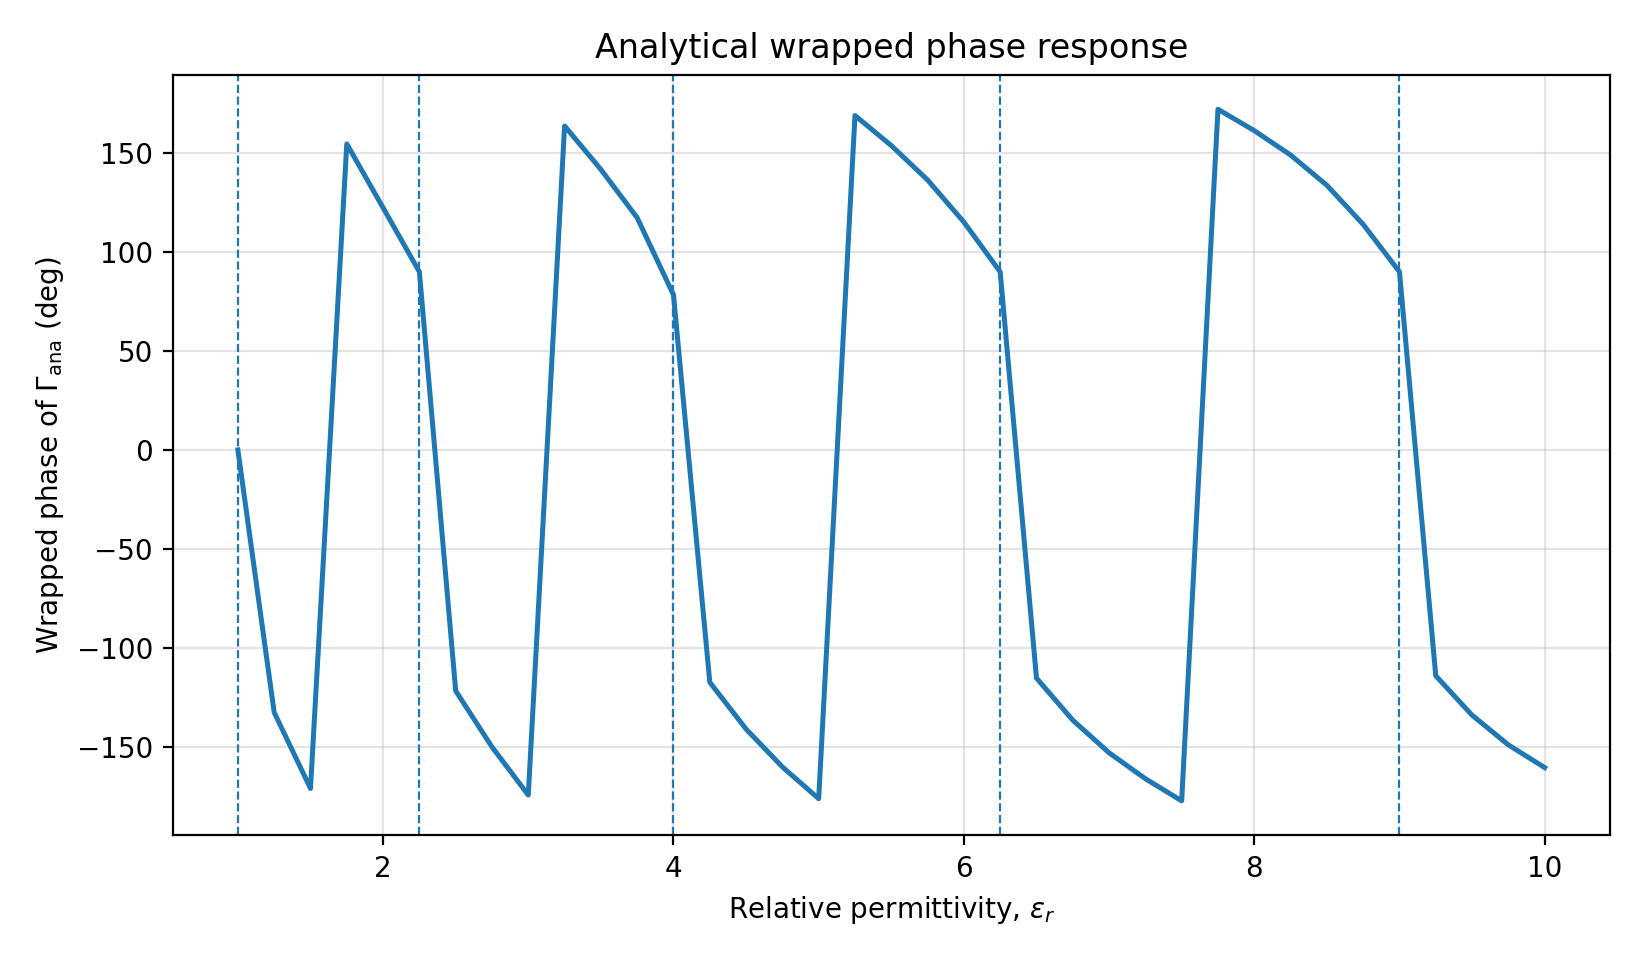
\includegraphics[width=0.88\textwidth]{figures/analytical/analytical_phase_vs_eps.png}
    \caption{Regenerated wrapped analytical phase. Values at or extremely near the
    reflection zeros are numerically sensitive and are not used as matching metrics.}
    \label{fig:analytical-phase}
\end{figure}
